\subsubsubsubsection{Infrastracture director}
\begin{figure}[h]
\centering
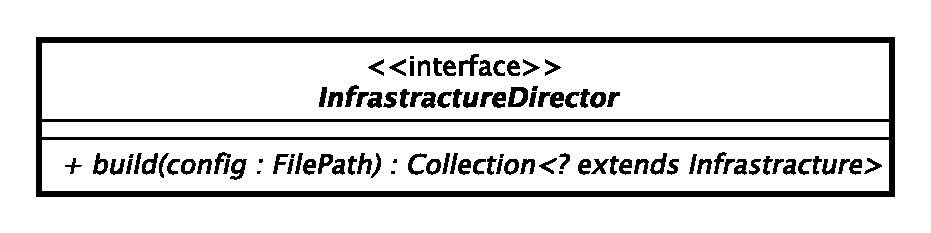
\includegraphics[scale=0.6,keepaspectratio]{images/solution/app/backend/infrastracture_director.eps}
\caption{\pReactiveBuild::InfrastractureDirector}
\label{fig:sd-app-infrastracture-director}
\end{figure}
\FloatBarrier
\begin{itemize}
  \item \textbf{\descr} \\
    It represents the urban infrastracture component director which instructs the builder.
  \item \textbf{\ops}
  \begin{itemize} 
    \item[+] \texttt{\textit{build(config: FilePath) : Collection<? extends Infrastracture>}} \\
Builds a collection of urban entities according to the configuration file. It uses the
builder multiple times to create incrementally a configuration of the requested
urban infrastracture component as specified in the configuration file.
  \end{itemize}
\end{itemize}
